
% Begin with describing virtual circuit switching
\begin{section}{Introduction: Packet Scheduling in Switches}
Packet switches and routers use a switched backplane based on simple 2x2 crossbar switches. Most often, these systems use input queues to hold incoming packets waiting to get switched through the switching fabric to their destined output ports. The packet scheduling \& queueing algorithm used for this can greatly affect the performance of the switch. This assignment explores the popular iSLIP algorithm and compares them to classical No-Queuing (NOQ) and Input Queueing with Head-of-Line Blocking cases.
\end{section}


\begin{section}{Challenges}
 Input Queueing with a simple First-In First-Out scheduling is known to suffer from Head-of-Line blocking effect in which, a blockage at the HOL make all the subsequent waiting packets in the queue suffer. Further, while guaranteeing high utilisation and low drop probability, the scheduling algorithm must also respect flow-wise packet order, guarantee fairness and must adapt quickly to changes in the traffic or bursts in the network. All these challenges, make it difficult to design scheduling algorithms for packet switches. 
\end{section}

\begin{section}{Simulation Experiment}
    This experiment designs a switch simulator to test out different scheduling algorithms, and compares their drop probabilities, delays and link utilisation. Further the simulator is flexible to handle many different parameters and is easily extensible to other scheduling algorithms.
\end{section}

\begin{section}{Variables of the Experiment}
    \begin{subsection}{Number of Switch Ports $N$}
        The switch is assumed to have $N$ input ports and $N$ output ports, numbered from $0$ to $N-1$. The default value is $8$.
    \end{subsection}
    
    \begin{subsection}{Buffer Size $B$}
        Each input and output port can hold up to $B$ fixed-length packets. The default value is $10$.
    \end{subsection}
    
    \begin{subsection}{Packet Generation Probability $p$}
        Each input port generates a packet in a time slot according to a Bernoulli$(p)$ distribution, where $p$ denotes the probability that a packet is generated. The default value is $0.5$.
    \end{subsection}
    
    \begin{subsection}{Queue Type $q$}
        This argument specifies the type of queue used for packet handling. Possible values include NOQ (No Queuing), INQ (Input Queuing), and CIOQ (Combined Input and Output Queuing). The default queue type is INQ.
    \end{subsection}
    
    \begin{subsection}{Knockout $K$}
        This parameter is specific to the CIOQ queue type and determines the backplane speedup compared to the output link transmission time. $K=2$ means that in one transmission time unit of the output port, the backplane can switch two rounds of packets. The default value is $1$.
    \end{subsection}
    
    \begin{subsection}{Input Queue Length Lookahead $L$}
        This parameter is also specific to the CIOQ queue type and defines the length of the input queue to be considered for packet scheduling. $L=B$ means that all the packets in the input queue will be considered for scheduling. The default value is $1$.
    \end{subsection}
    
    \begin{subsection}{Maximum Slots $T$}
        This argument specifies the total number of time slots for the simulation. Each time slot corresponds to the transmission time of one packet. The default value is $10,000$.
    \end{subsection}

\end{section}

\newpage
\begin{section}{iSLIP Algorithm \cite{769767}}

    \begin{subsection}{Algorithm}
        \begin{algorithm}[h!]
            \caption{iSLIP Algorithm}
            \begin{algorithmic}[1]
                \State \textbf{Initialize:} All inputs and outputs are unmatched
                \Repeat
                    \State \textbf{Step 1: Request}
                    \For{each unmatched input}
                        \For{each output with a queued cell}
                            \State Send a request to the output
                        \EndFor
                    \EndFor
                    
                    \State \textbf{Step 2: Grant}
                    \For{each unmatched output}
                        \If{output received requests}
                            \State Grant to the next input in round robin order
                        \EndIf
                    \EndFor
                    
                    \State \textbf{Step 3: Accept}
                    \For{each unmatched input}
                        \If{input receives a grant}
                            \State Accept the grant in round robin order
                            \State Update round robin pointers for both input and output
                        \EndIf
                    \EndFor
                \Until{no change in schedule}
            \end{algorithmic}
        \end{algorithm}
    \end{subsection}

    \begin{subsection}{Time Complexity}
        Using various simualations with a $N\times N$ switch, the authors suggest that the iSLIP algorithm converges in $\log_2 N$ steps \cite{1}. However, they have not been able to prove the bound $\mathbf{E}(I) \leq log_2 N$. 
        Note that this is a much faster algorithm that classical Maximum Weight Matching scheduling algorithm which requires $\mathcal{O}(N^3)$ time to converge, and has time complexity comparable to Parallel Iterative Matching algorithm which is proved to converge within $\log_2 N + \frac{4}{3}$ iterations on average \cite{1} .
    \end{subsection}

    \begin{subsection}{Salient Features}

    \end{subsection}

    \begin{subsection}{Example Run}
        Consider the following example for the iSLIP algorithm. Initial state of all the input queues is shown below. Assume that initially all the round robin (RR) pointer are initialised to 0. Ports are considered to be 0-indexed, that is, after a packet from the $i$th input port is accepted to the $j$th output port, the RR pointer of the $i$th input port will be set to $j$ and the RR pointer of the $j$th output port will be set to $i$. For this example, $N=4$ and $L=2$, that is, the first two packets in each port is considered by the algorithm.\\

        \begin{table}[h!]
            \centering
            \caption{Initial State of the Switch}
            \begin{tabular}{|c|c|c|c|c|}
                \hline
                \textbf{Input Port} & \textbf{Queue State} & \textbf{RR Pointer (Input)} & \textbf{RR Pointer (Output)} \\ \hline
                0 & [Packet 1, Packet 2] & 0 & 0 \\ \hline
                1 & [Packet 3, Packet 2] & 0 & 0 \\ \hline
                2 & [Packet 3, Packet 0] & 0 & 0 \\ \hline
                3 & [Packet 0, Packet 1] & 0 & 0 \\ \hline
            \end{tabular}
            \label{tab:switch_state}
        \end{table}

        In the first iteration these are the grants received each output port and the acceptances issued by each input port. 

        \begin{table}[h!]
            \centering
            \caption{Grants Received and Acceptances Issued in the First Iteration}
            \begin{tabular}{|c|c|c|c|}
                \hline
                \textbf{Output Port} & \textbf{Grant Received From} & \textbf{Input Port} & \textbf{Accepts Received} \\ \hline
                0 & Input Port 2 and 3 & 0 & Output Port 1 and 2 (1 accepted) \\ \hline
                1 & Input Port 0 and 3 & 1 & Output port 3 (3 accepted)\\ \hline
                2 & Input Port 0 and 1 & 2 & Output Port 0 (0 accepted)\\ \hline
                3 & Input Port 1 and 2 & 3 & None \\ \hline
            \end{tabular}
            \label{tab:grants_acceptances}
        \end{table}

        As we can see, each Output ports receives two grants, for each of the two packets stored among the $NL$ packets in the input queues, destined to that particular output port. Each output port then selects the next packet in RR fashion after the RR pointer and sends a accept request to the corresponding input port. Each input port then selects the next packet in RR fashion again according to its own RR pointers. \\
        Thus after this iteration, the matching of input and output ports is ${(0, 1), (1, 3), (2, 0)}$. Thus the corresponding RR pointers of the ports are updated as follows:

        \begin{table}[h!]
            \centering
            \caption{Initial State of the Switch}
            \begin{tabular}{|c|c|c|c|c|}
                \hline
                \textbf{Input Port} & \textbf{Queue State} & \textbf{RR Pointer (Input)} & \textbf{RR Pointer (Output)} \\ \hline
                0 & [\sout{Packet 1}, Packet 2] & 1 & 2 \\ \hline
                1 & [\sout{Packet 3}, Packet 2] & 3 & 0 \\ \hline
                2 & [Packet 3, \sout{Packet 0}] & 0 & 0 \\ \hline
                3 & [Packet 0, Packet 1] & 0 & 1 \\ \hline
            \end{tabular}
            \label{tab:switch_state}
        \end{table}

        In the next iteration, only the input ports, and the output ports which are not yet matched are considered. The grant table is described below:


        \begin{table}[h!]
            \centering
            \caption{Grants Received and Acceptances Issued in the First Iteration}
            \begin{tabular}{|c|c|c|c|}
                \hline
                \textbf{Output Port} & \textbf{Grant Received From} & \textbf{Input Port} & \textbf{Accepts Received} \\ \hline
                0 & Input Port 3 & 0 & None \\ \hline
                1 & Input Port 3 & 1 & None\\ \hline
                2 & None & 2 & None \\ \hline
                3 & None & 3 & None \\ \hline
            \end{tabular}
            \label{tab:grants_acceptances}
        \end{table}

        Since the output ports which received the grants are already matched, there are no Acceptance issued, and the matching remains unaltered. Thus, the iterations stop and the following mapping of ports is output.

\begin{table}[h!]
    \centering
    \caption{Final Mapping of Input and Output Ports}
    \begin{tabular}{|c|c|}
        \hline
        \textbf{Input Port} & \textbf{Output Port} \\ \hline
        0 & 1 \\ \hline
        1 & 3 \\ \hline
        2 & 0 \\ \hline
        3 & None \\ \hline
    \end{tabular}
    \label{tab:final_mapping}
\end{table}


    \end{subsection}

\end{section}


\begin{section}{Results}

    \begin{subsection}{Comparison with different probabilities}

    \begin{figure}[h!]
        \centering
        % First figure (fig1a)
        \begin{subfigure}[b]{0.45\textwidth}
            \centering
            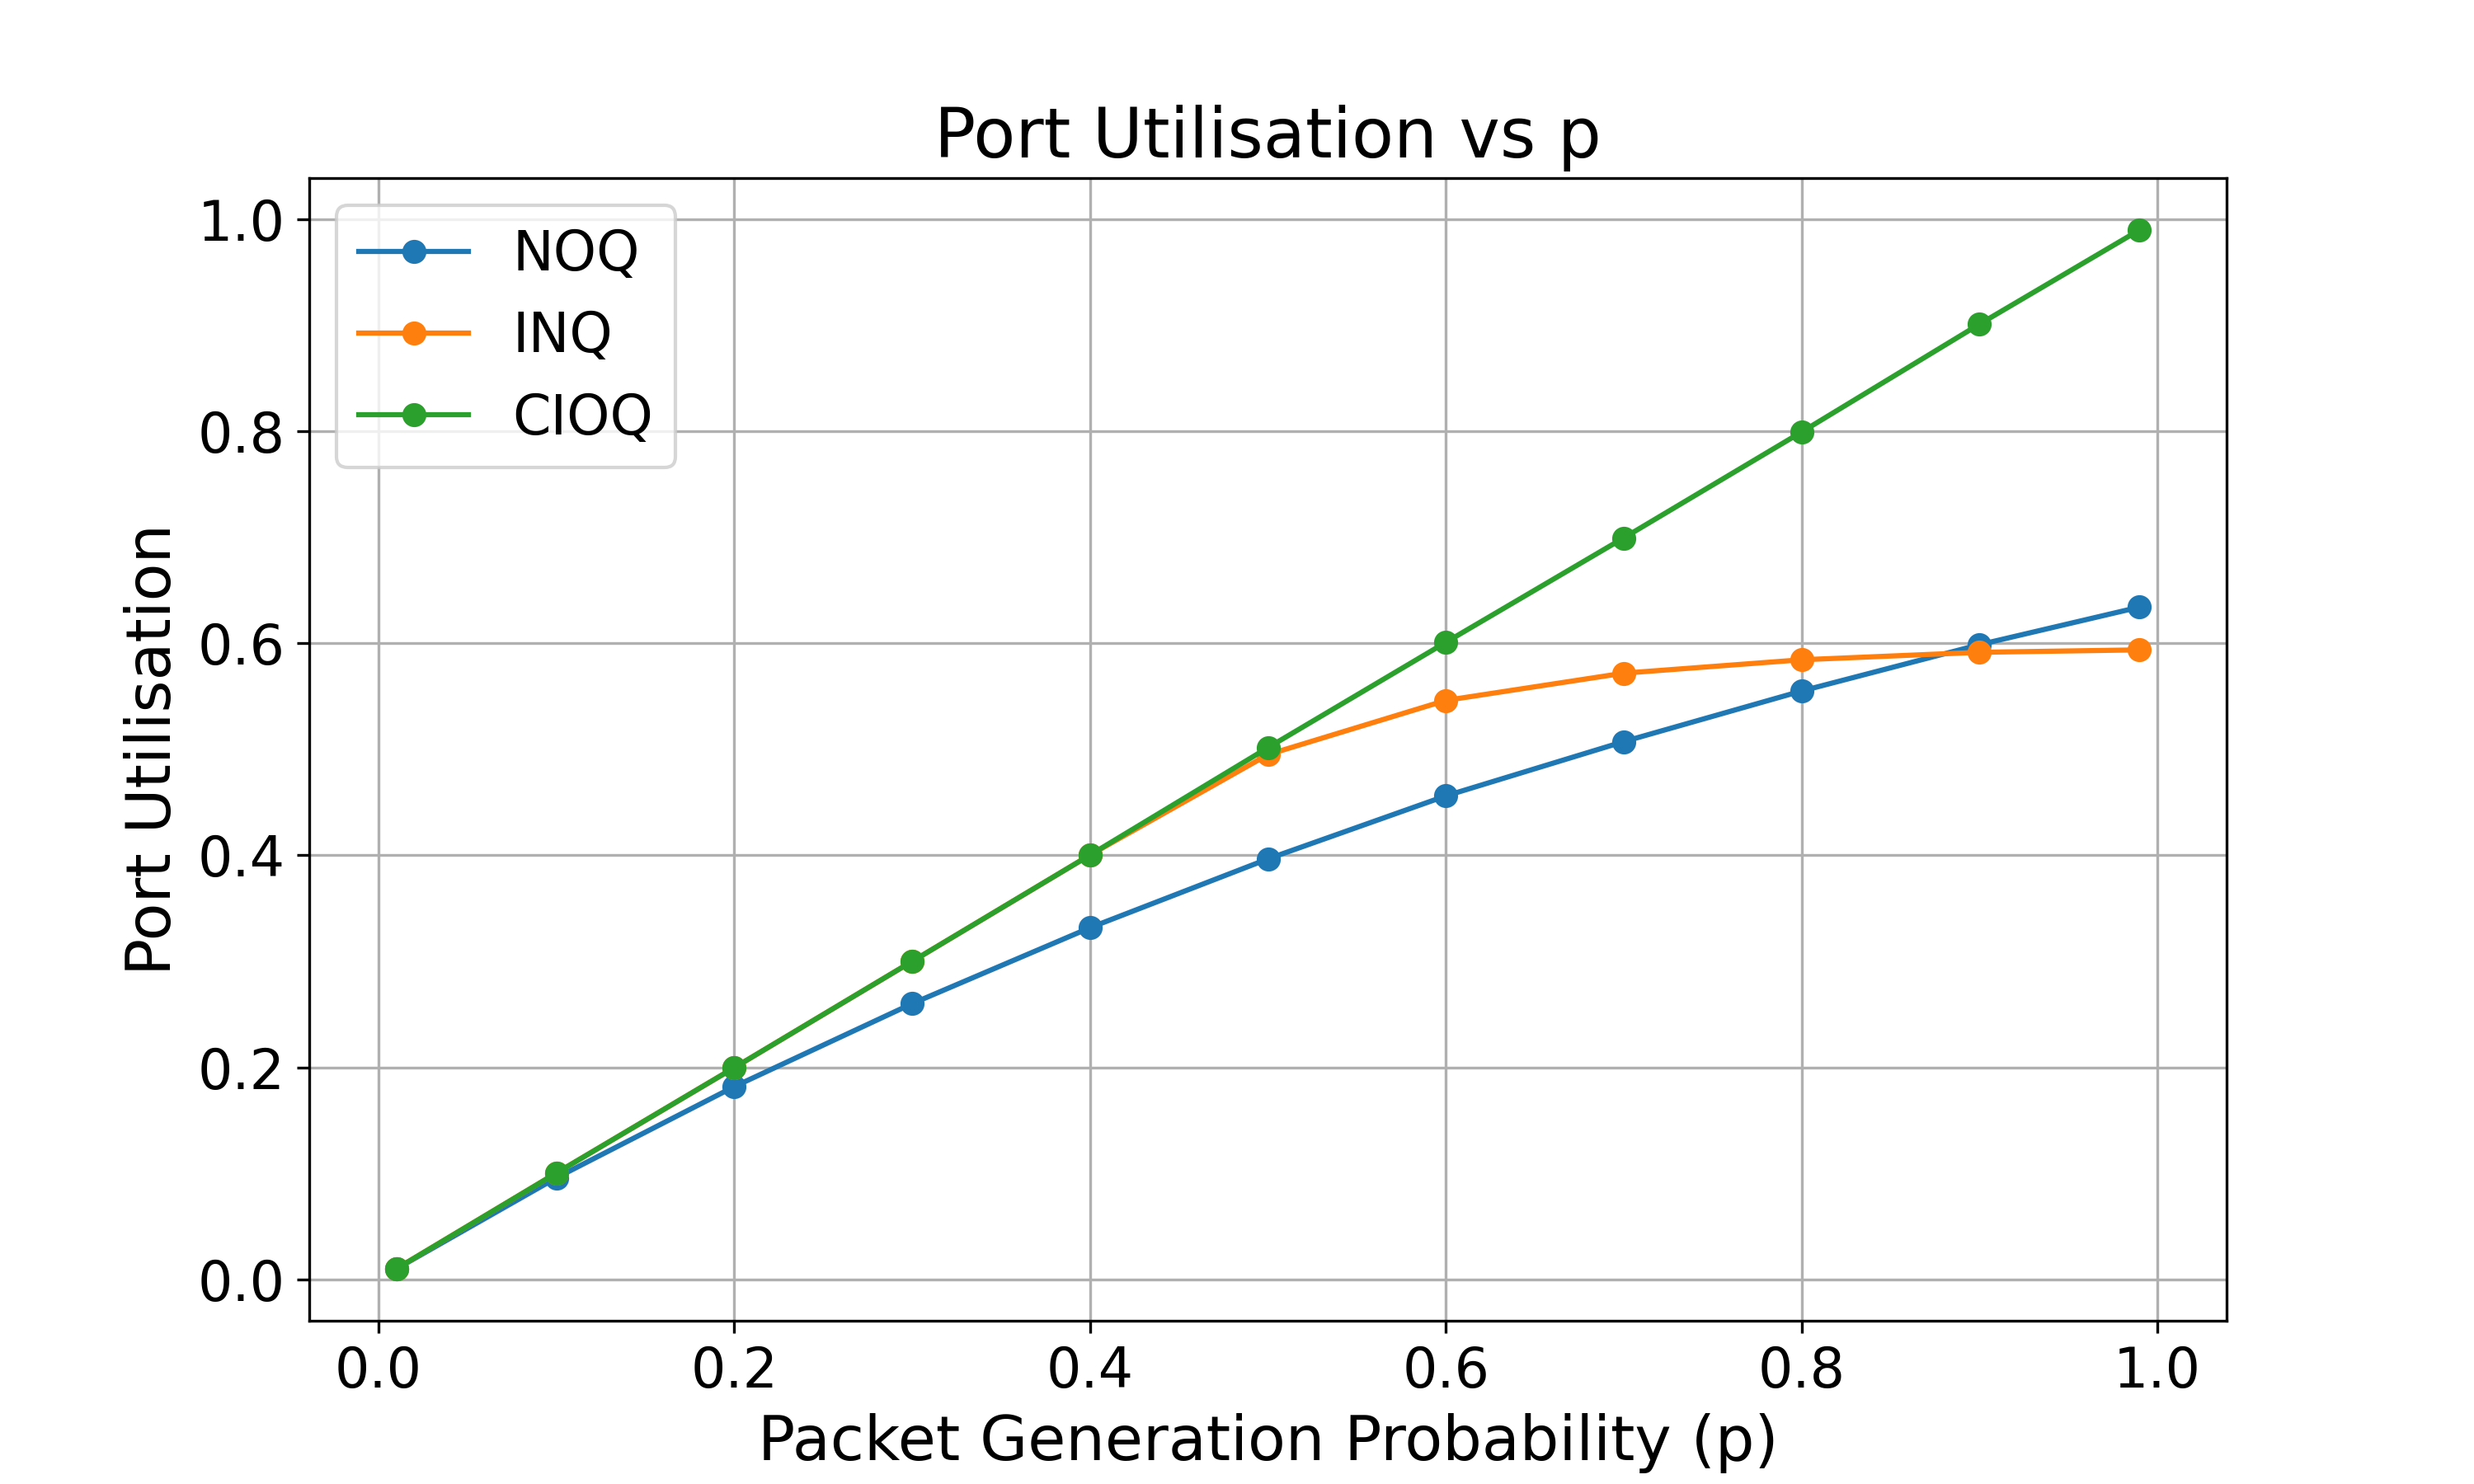
\includegraphics[width=\textwidth]{figures/fig1/fig1a.png}
        \end{subfigure}
        \hfill
        % Second figure (figures/fig1/fig1b)
        \begin{subfigure}[b]{0.45\textwidth}
            \centering
            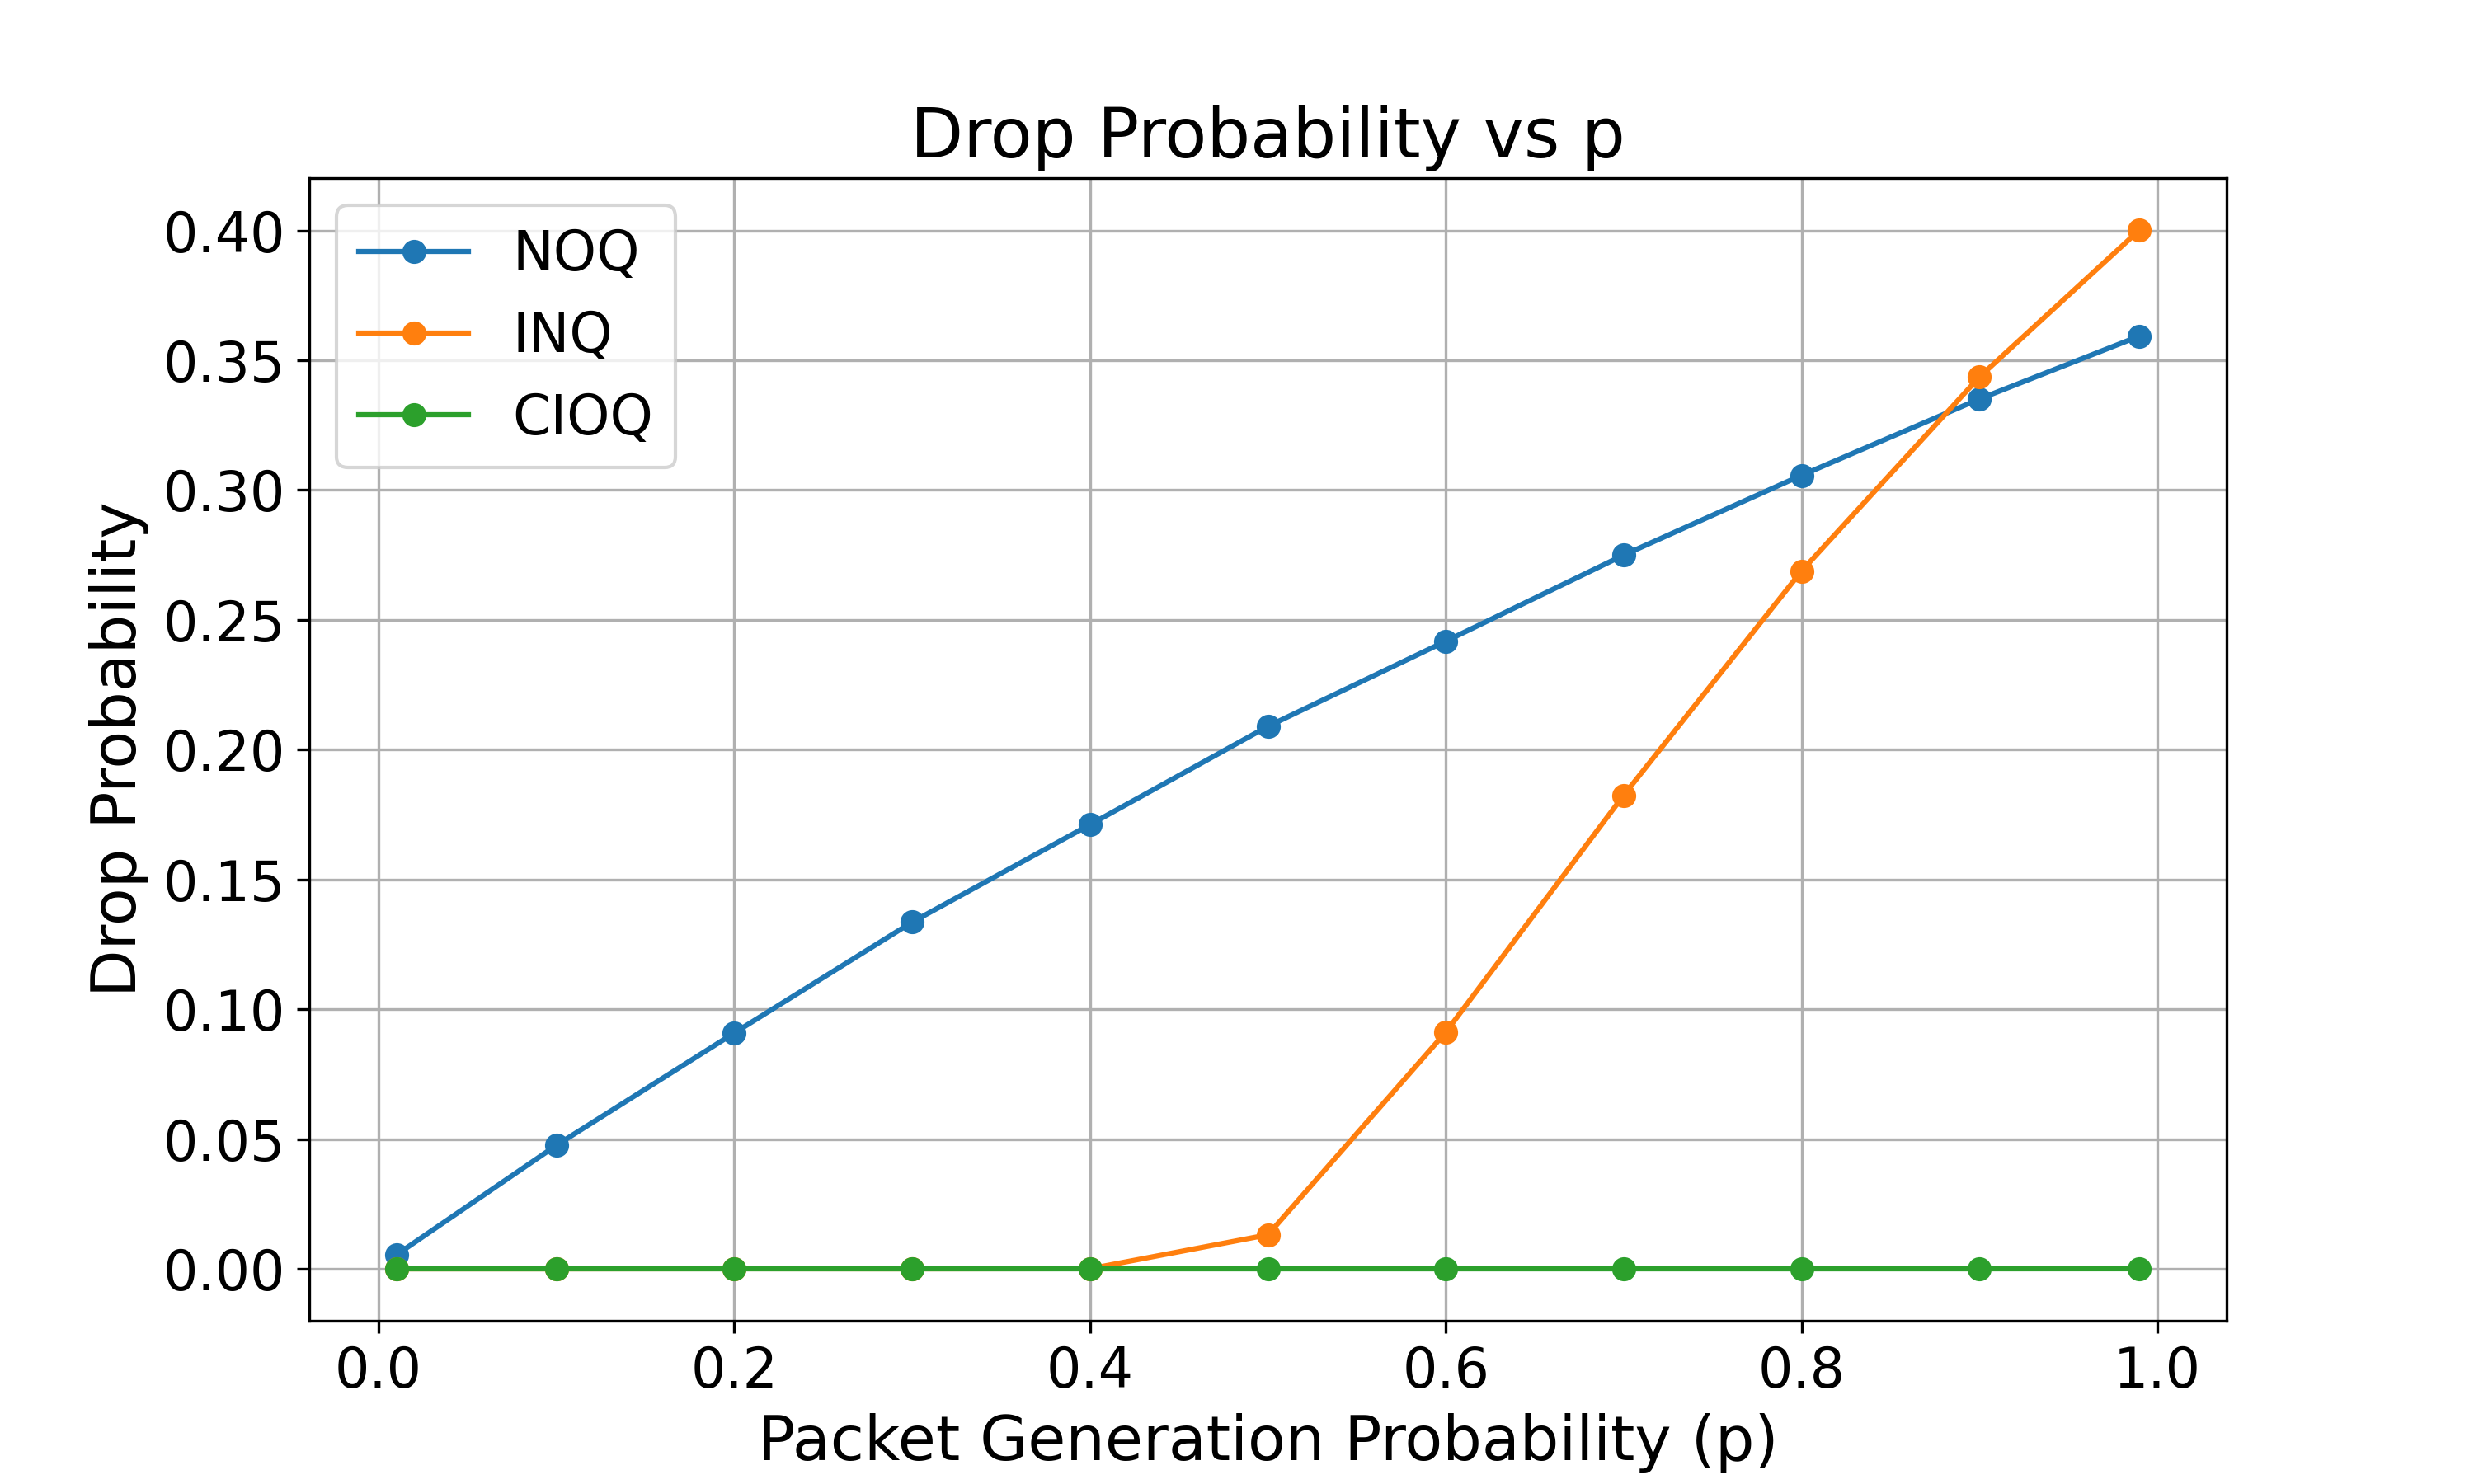
\includegraphics[width=\textwidth]{figures/fig1/fig1b.png}
        \end{subfigure}
        \hfill
        % Third figure (figures/fig1/fig1c)
        \begin{subfigure}[b]{0.45\textwidth}
            \centering
            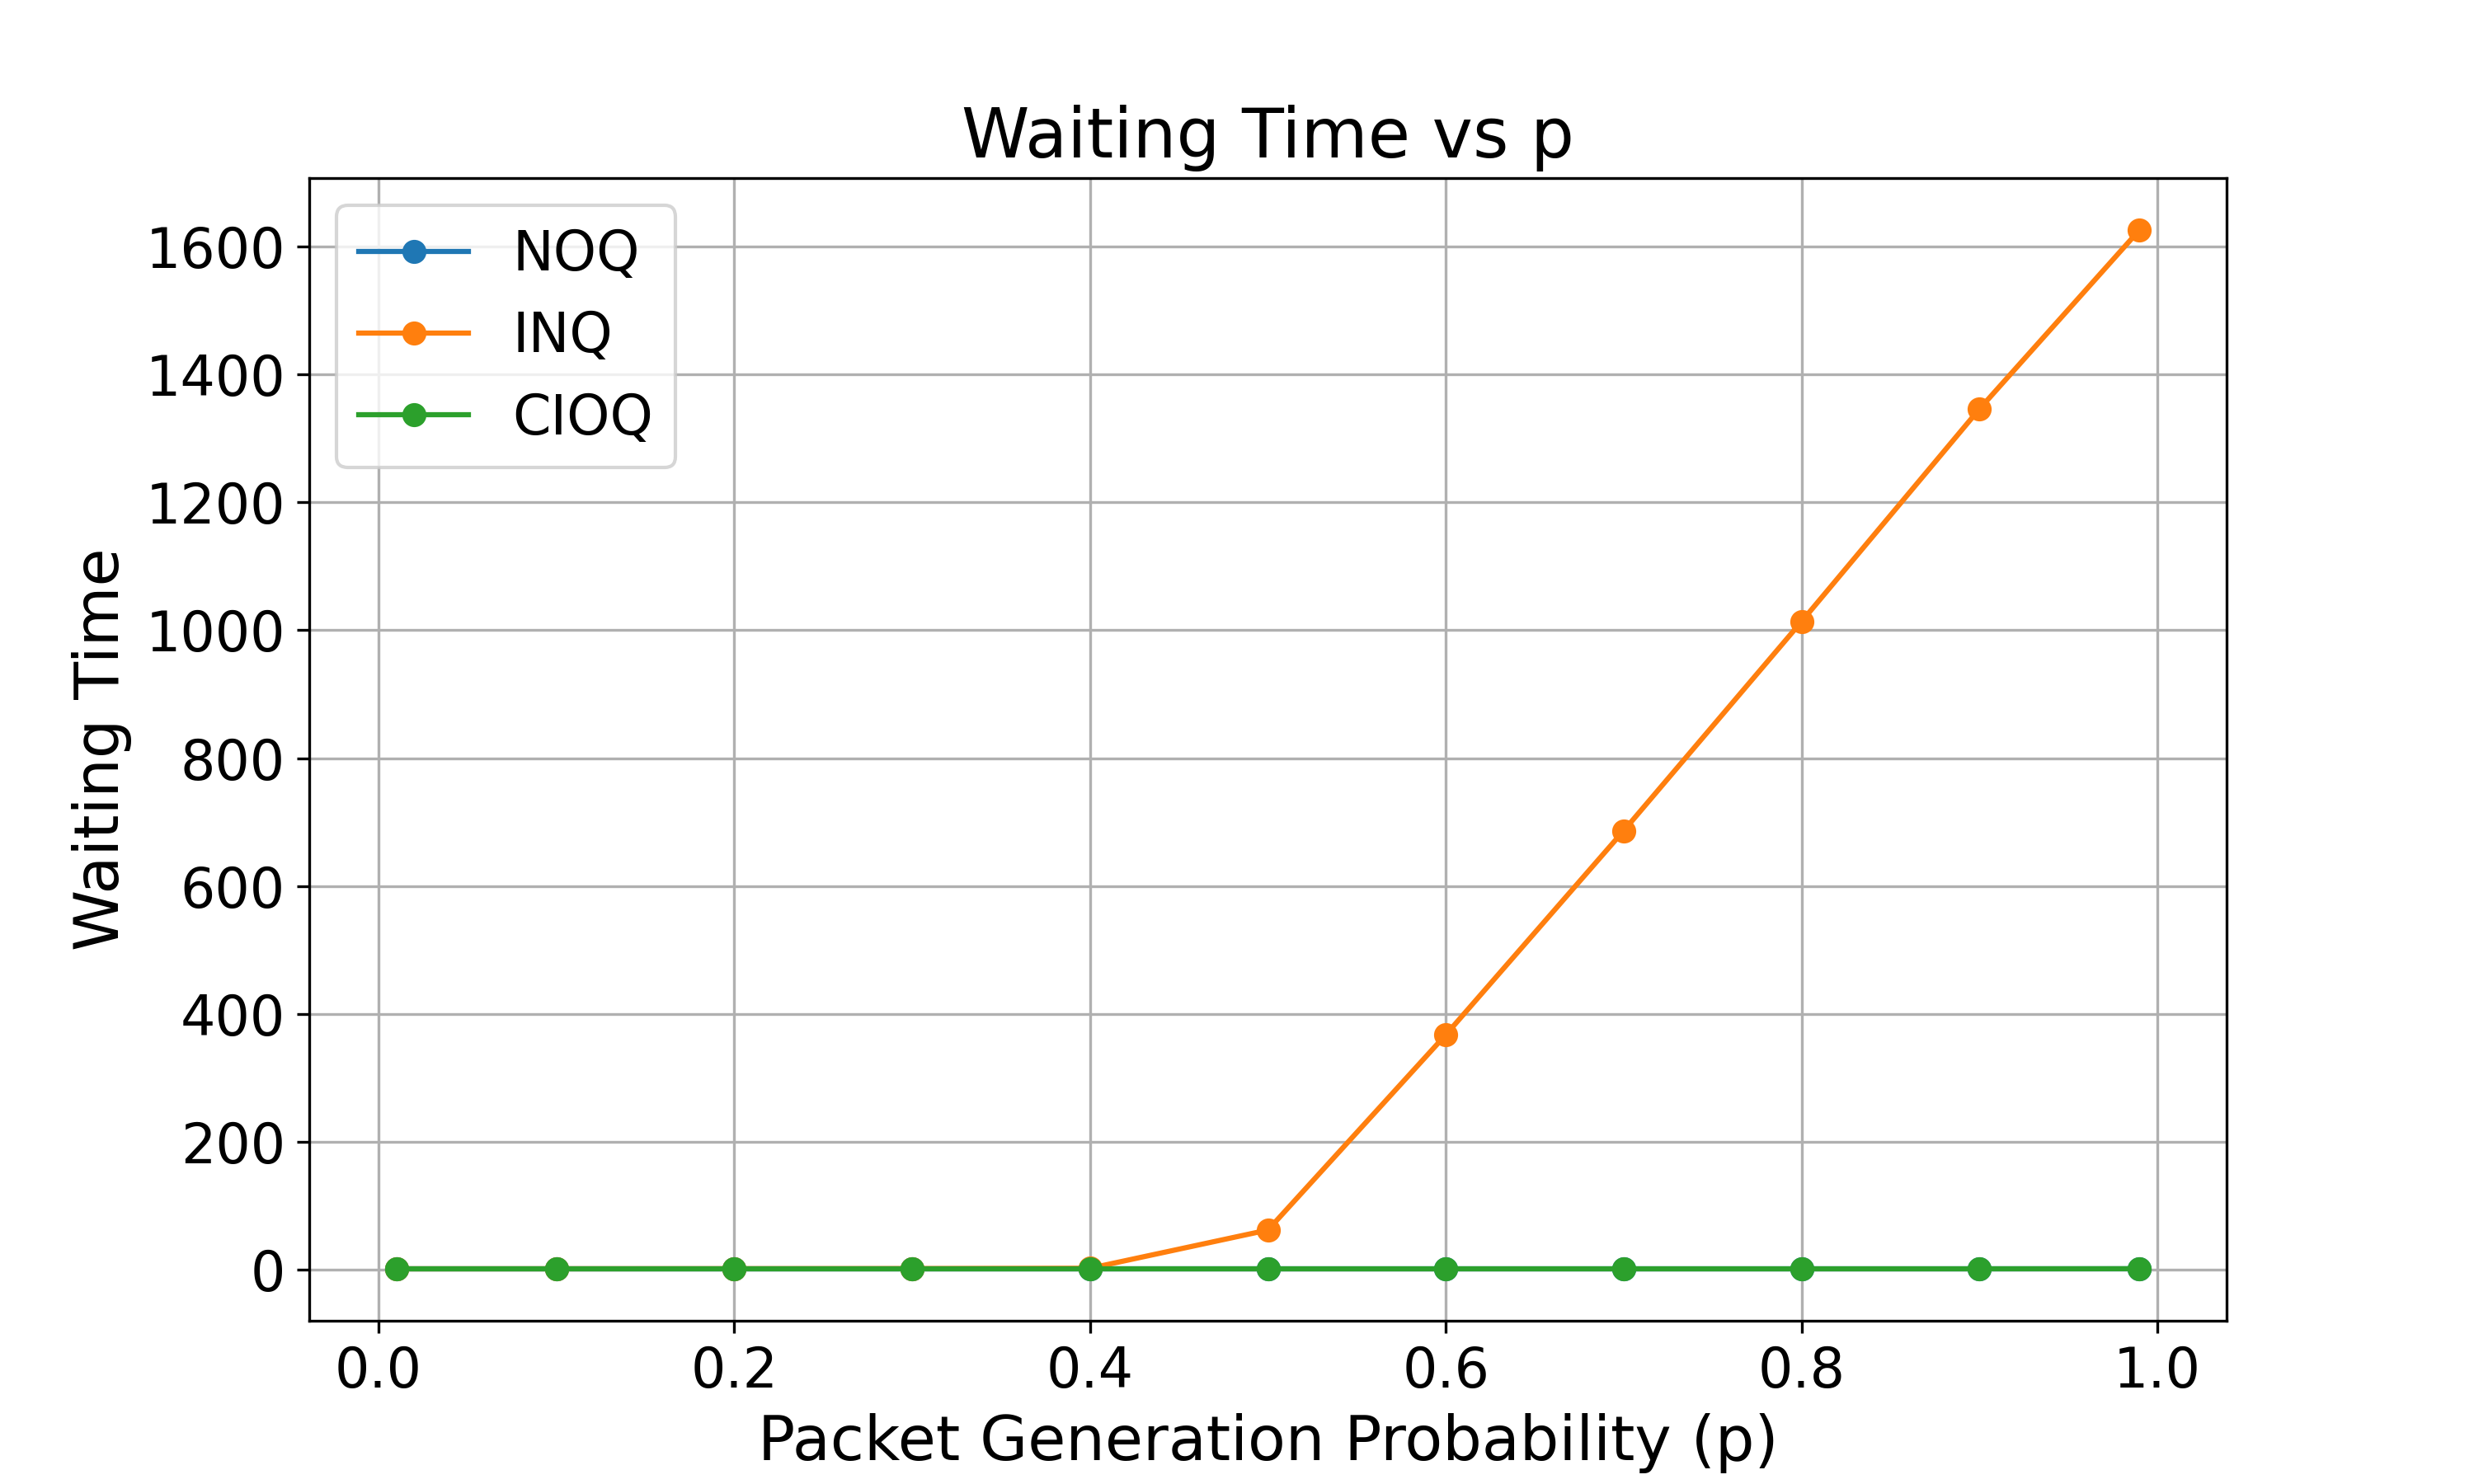
\includegraphics[width=\textwidth]{figures/fig1/fig1c.png}
        \end{subfigure}
        
        \caption{Comparing the different Queueing algorithms}
        \label{fig:combined}
    \end{figure}

    The above figure compares the link utilisation, drop probability and waiting time for the different algorithms with default parameters. For CIOQ, $K=4$ and $L=6$ was chosen. 
    \begin{subsubsection}{Utilisation}
        From the figure we see that iSLIP algorithm has the best utilisation and increasing linearly with the increase in probability. Also we see that the values for $p=1$ \textbf{agree with the theoretical maximum utilisation of $64\%$ for NOQ and $58.6\%$ for INQ}.
        One important insight from this is that although NOQ outperforms INQ, at lower loads, the INQ gives a much better utilisation than NOQ. 
    \end{subsubsection}

    \begin{subsubsection}{Drop Probability}
        CIOQ with iSLIP algorithm has as a consistent nearly 0 drop probability, whereas NOQ and IOQ have drop probabilities reaching to upto 40\% for $p=1$. Again, here INQ outperforms NOQ under low loads, but becomes worse under higher loads.
    \end{subsubsection}

    \begin{subsubsection}{Waiting Time}
    The waiting time for NOQ and CIOQ is consistently 1 time slot. But for INQ, the wait time increase approximately linearly after $p=0.5$, and reached a maximum of 1600 time slots. Thus, considering waiting time as the metric, NOQ and CIOQ are preferred.
    \end{subsubsection}

\end{subsection}

\begin{subsection}{Performance Graphs}
    The following graphs show the performance of the three algorithms for the following values:
    \begin{multicols}{2}
        \begin{itemize}
            \item Number of Ports (\(N\)):
            \begin{itemize}
                \item \(N = 32\)
                \item \(N = 64\)
            \end{itemize}
            \item Packet Generation Probability (\(p\)):
            \begin{itemize}
                \item \(p \in \{0.4, 0.6, 0.8, 1.0\}\)
            \end{itemize}
        \end{itemize}

        \begin{itemize}
            \item Parameter \(K\) for CIOQ:
            \begin{itemize}
                \item \(K \in \{0.4, 0.7, 1.0\} \times N\)
            \end{itemize}
            \item Parameter \(L\) for CIOQ:
            \begin{itemize}
                \item \(L \in \{0.4, 0.7, 1.0\} \times N\)
            \end{itemize}
        \end{itemize}
    \end{multicols}

    \begin{figure}[htbp]
        \centering
        % For N=32
        \begin{subfigure}{0.45\textwidth}
            \centering
            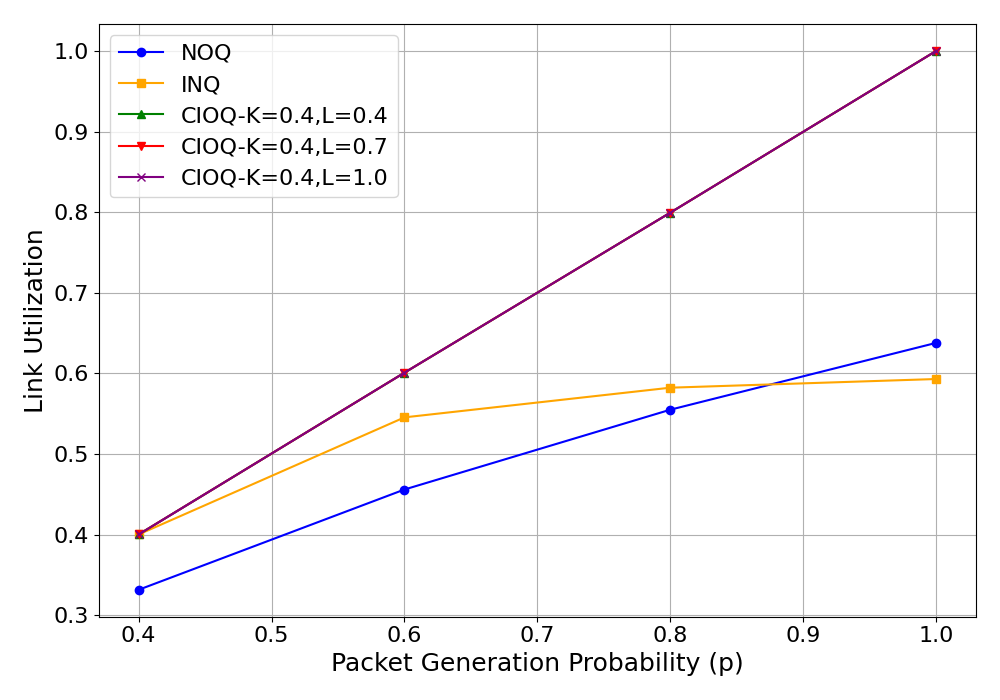
\includegraphics[width=\linewidth]{./figures/fig2/utilization_plot_N_32.png}
            \caption{Utilization for \(N = 32\)}
            \label{fig:utilization_32}
        \end{subfigure}
        \hfill
        \begin{subfigure}{0.45\textwidth}
            \centering
            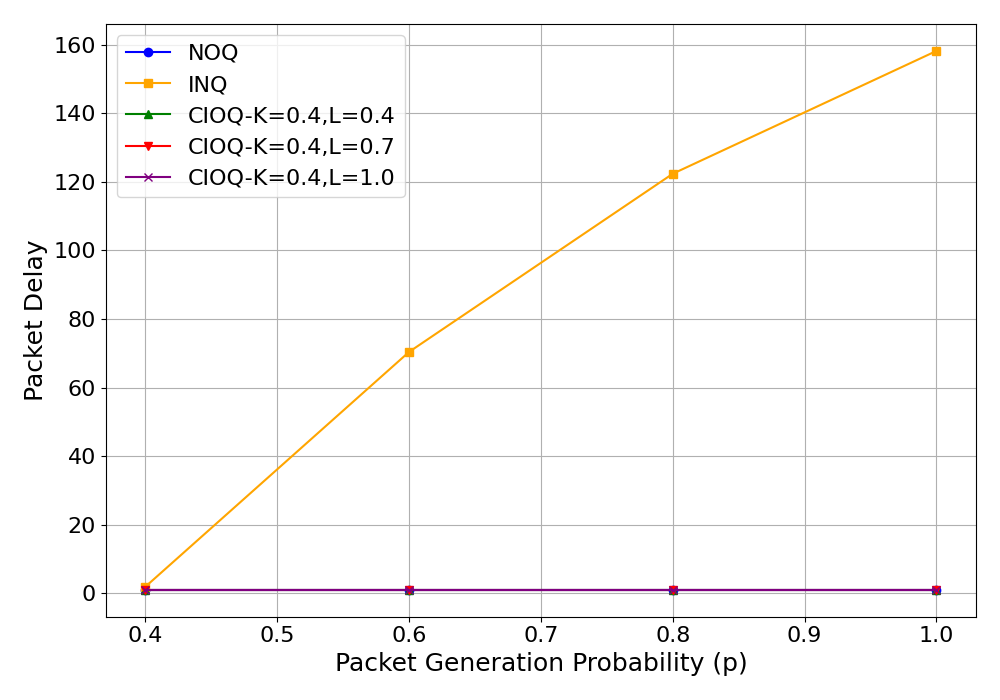
\includegraphics[width=\linewidth]{./figures/fig2/delay_plot_N_32.png}
            \caption{Delay for \(N = 32\)}
            \label{fig:delay_32}
        \end{subfigure}

        \vspace{0.5cm} % Space between rows

        % For N=64
        \begin{subfigure}{0.45\textwidth}
            \centering
            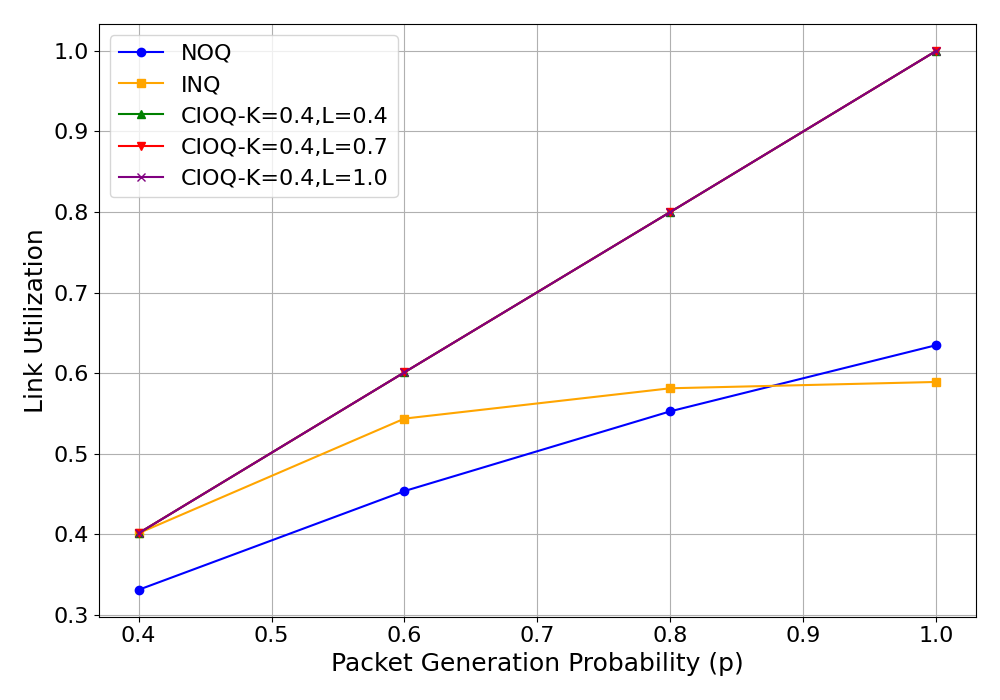
\includegraphics[width=\linewidth]{./figures/fig2/utilization_plot_N_64.png}
            \caption{Utilization for \(N = 64\)}
            \label{fig:utilization_64}
        \end{subfigure}
        \hfill
        \begin{subfigure}{0.45\textwidth}
            \centering
            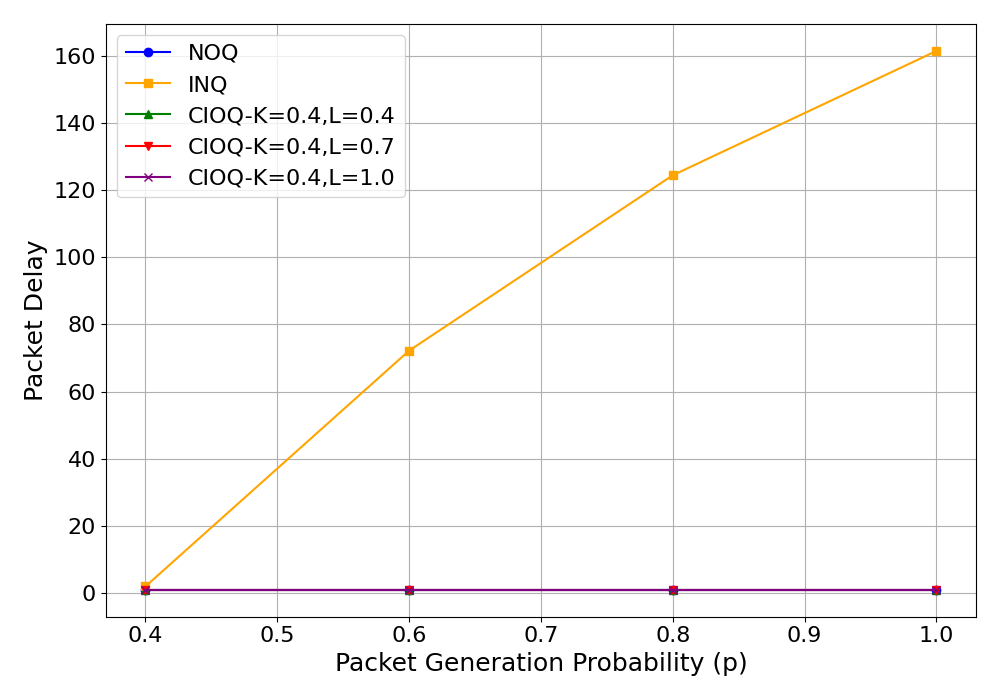
\includegraphics[width=\linewidth]{./figures/fig2/delay_plot_N_64.png}
            \caption{Delay for \(N = 64\)}
            \label{fig:delay_64}
        \end{subfigure}

        \caption{Performance graphs for different values of \(N\).}
        \label{fig:performance_graphs}
    \end{figure}
    
    The above graphs can be interpreted as follows:
    \begin{itemize}
        \item As depicted in the figure above, the CIOQ link utilisation and packet delay achieves maximum theoretical value of $p$ (that is, along $y=x$ line), and packet delay of $1$ for $K=0.4, L=0.4$ itself. Therefore, increasing $K$ or $L$ further will not improve the statistics any further. Thus, only a few curves for different values of $L$ is plotted for clarity sake. 
        \item As we can see from the figure above, the utilisation of CIOQ is best. For lower loads (values of $p$), INQ performs better than NOQ, but for higher values NOQ performs better. 
        \item We also see that the delay of CIOQ and NOQ both are 1, but for INQ, the delay increases a lot with higher values of $P$.
        \item Another important observation is that, for $N=32$ and $N=64$, the graphs are exactly identical. This is probably because we are comparing the averages over a long time period, with $T=10000$ time slots and a large buffer size of $100$.
    \end{itemize}

    \end{subsection}
    

\end{section}

\begin{section}{Conclusion}
    The iSLIP performs much better than No Queue (NOQ) and Input Queueing with FIFO scheduling (INQ) on link utilisation and drop probability metrics. Further it also achieves packet delays of nearly 1 time slot not unlike NOQ. Among INQ and NOQ, INQ suffers from much higher packet delays. At lesser loads, INQ outperforms NOQ in drop probability and link utilisation, but NOQ surpasses INQ at higher loads, as is expected from the theoretical results.  
\end{section}
